\documentclass[article]{jss}
\usepackage[utf8]{inputenc}

\providecommand{\tightlist}{%
  \setlength{\itemsep}{0pt}\setlength{\parskip}{0pt}}

\author{
Ursula Laa\\Monash University \And Second Author\\Affiliation
}
\title{Scagnostics and Projection Pursuit}

\Plainauthor{Ursula Laa, Second Author}

\Abstract{
The abstract of the article.
}

\Keywords{scagnostics, tour, projection pursuit}

%% publication information
%% \Volume{50}
%% \Issue{9}
%% \Month{June}
%% \Year{2012}
%% \Submitdate{}
%% \Acceptdate{2012-06-04}

\Address{
    Ursula Laa\\
  Monash University\\
  First line Second line\\
  E-mail: \email{ursula.laa@monash.edu}\\
  URL: \url{http://rstudio.com}\\~\\
    }

\usepackage{amsmath}

\begin{document}

\section{Introduction}\label{introduction}

A grand tour provides dynamic projections from the high dimensions into
some low dimensional representation, in particular also as a two
dimensional scatter plot ADDREF. The idea of projection persuit can be
coupled to the tour algorithm, to guide the tour towards more
interesting views of the projected data (the so-called guided tour), by
maximising a given projection persuit index ADDREF (Cook, Buja, Cabrera,
Hurley, 1995). The guided tour thus allows the user to view interesting
projections (local maxima or minima of given index) as well as their
neighborhoods, allowing the user to see the projection in the context of
the full parameter space. Typically projection persuit indices are built
to detect deviations of the projected data from a normal distribution,
and the nonnormalness is considered equivalent to interestingness of a
given projection ADDREF (Cook, Buja, Cabrera, 1993). Moreover, indices
for detecting holes, concentration of mass in the center or skewness
have also been designed.

Here we aim to extend the definition of interesting projections and
available projection persuit indices by studying potential new index
functions. As a starting point we consdier the scagnostics measures that
were proposed for selecting bivariate scatterplots in high-dimensional
datasets ADDREF (??). Rather than considering the scagnostics measures
for all possible bivariate combinations, we want to use one of the
measures as an index function for a guided tour of 2 dimensional
projections. We first study the feasability of this approach and discuss
potential pitfalls. We then aim to define more robust measures \ldots{}
???

\section{Scagnostics measures}\label{scagnostics-measures}

Eight scagnostics measures have been defined, the definitions are based
on the convex and alpha hull as well as the minimum spanning tree. Give
definitions here\ldots{}

Note that in practice the measures are calculated after binning the data
to avoid large computing times.

\section{Analysis setup}\label{analysis-setup}

To study the feasablility of using scagnostics measures as an index
fuction for guided tours, we first consider the variation of each of the
measures, as calculated from the projected scatter plot, when smoothly
changing the projection via the tour algorithm. Moreover, we test the
dependence on the sample size and on the outlier removal typically
performed to make the scagnostics measures more robust. In addition the
computing time is also important, as it might limit the dynamic viewing
and require to first record a guided tour path which can later be viewed
in a smooth display.

As we will see the scagnostics measures often exhibit a significant jump
despite changing smoothly between projections, a consequence of the
discreete nature of the definition, but possibly also due to the binning
performed as a first step of calculation. We therefore explore options
of ameliorating this situation using different smoothing methods, and by
redefining the measures in a more robust fashion.

\section{Application to particle physics
data}\label{application-to-particle-physics-data}

\subsection{Data description}\label{data-description}

For the following illustrations we work with the particle physics
dataset (ATLAS Collaboration, 2015). This data includes a number of
predictions for observables (in agreement with current limits) and the
so-called finetuning measure for a large set of parameter points in a
supersymmetric model. The observables describe predictions for decay
branching ratios and other precision observables that are generally used
to constrain new models of particle physics. We use the log transformed
values for the variables XYZ but not the finetuning, and we rescale all
variables to a {[}0,1{]} interval to obtain comparable scales.
Contributions to the variable gminus2 can be negative or positive, we
therefore add a small shift before the log transformation of this
variable.

\subsection{Software setup}\label{software-setup}

Use tourr and scagnostics package (ADDREF)

\subsection{Scagnositics of grand tour
projections}\label{scagnositics-of-grand-tour-projections}

\begin{CodeChunk}
\begin{figure}

{\centering 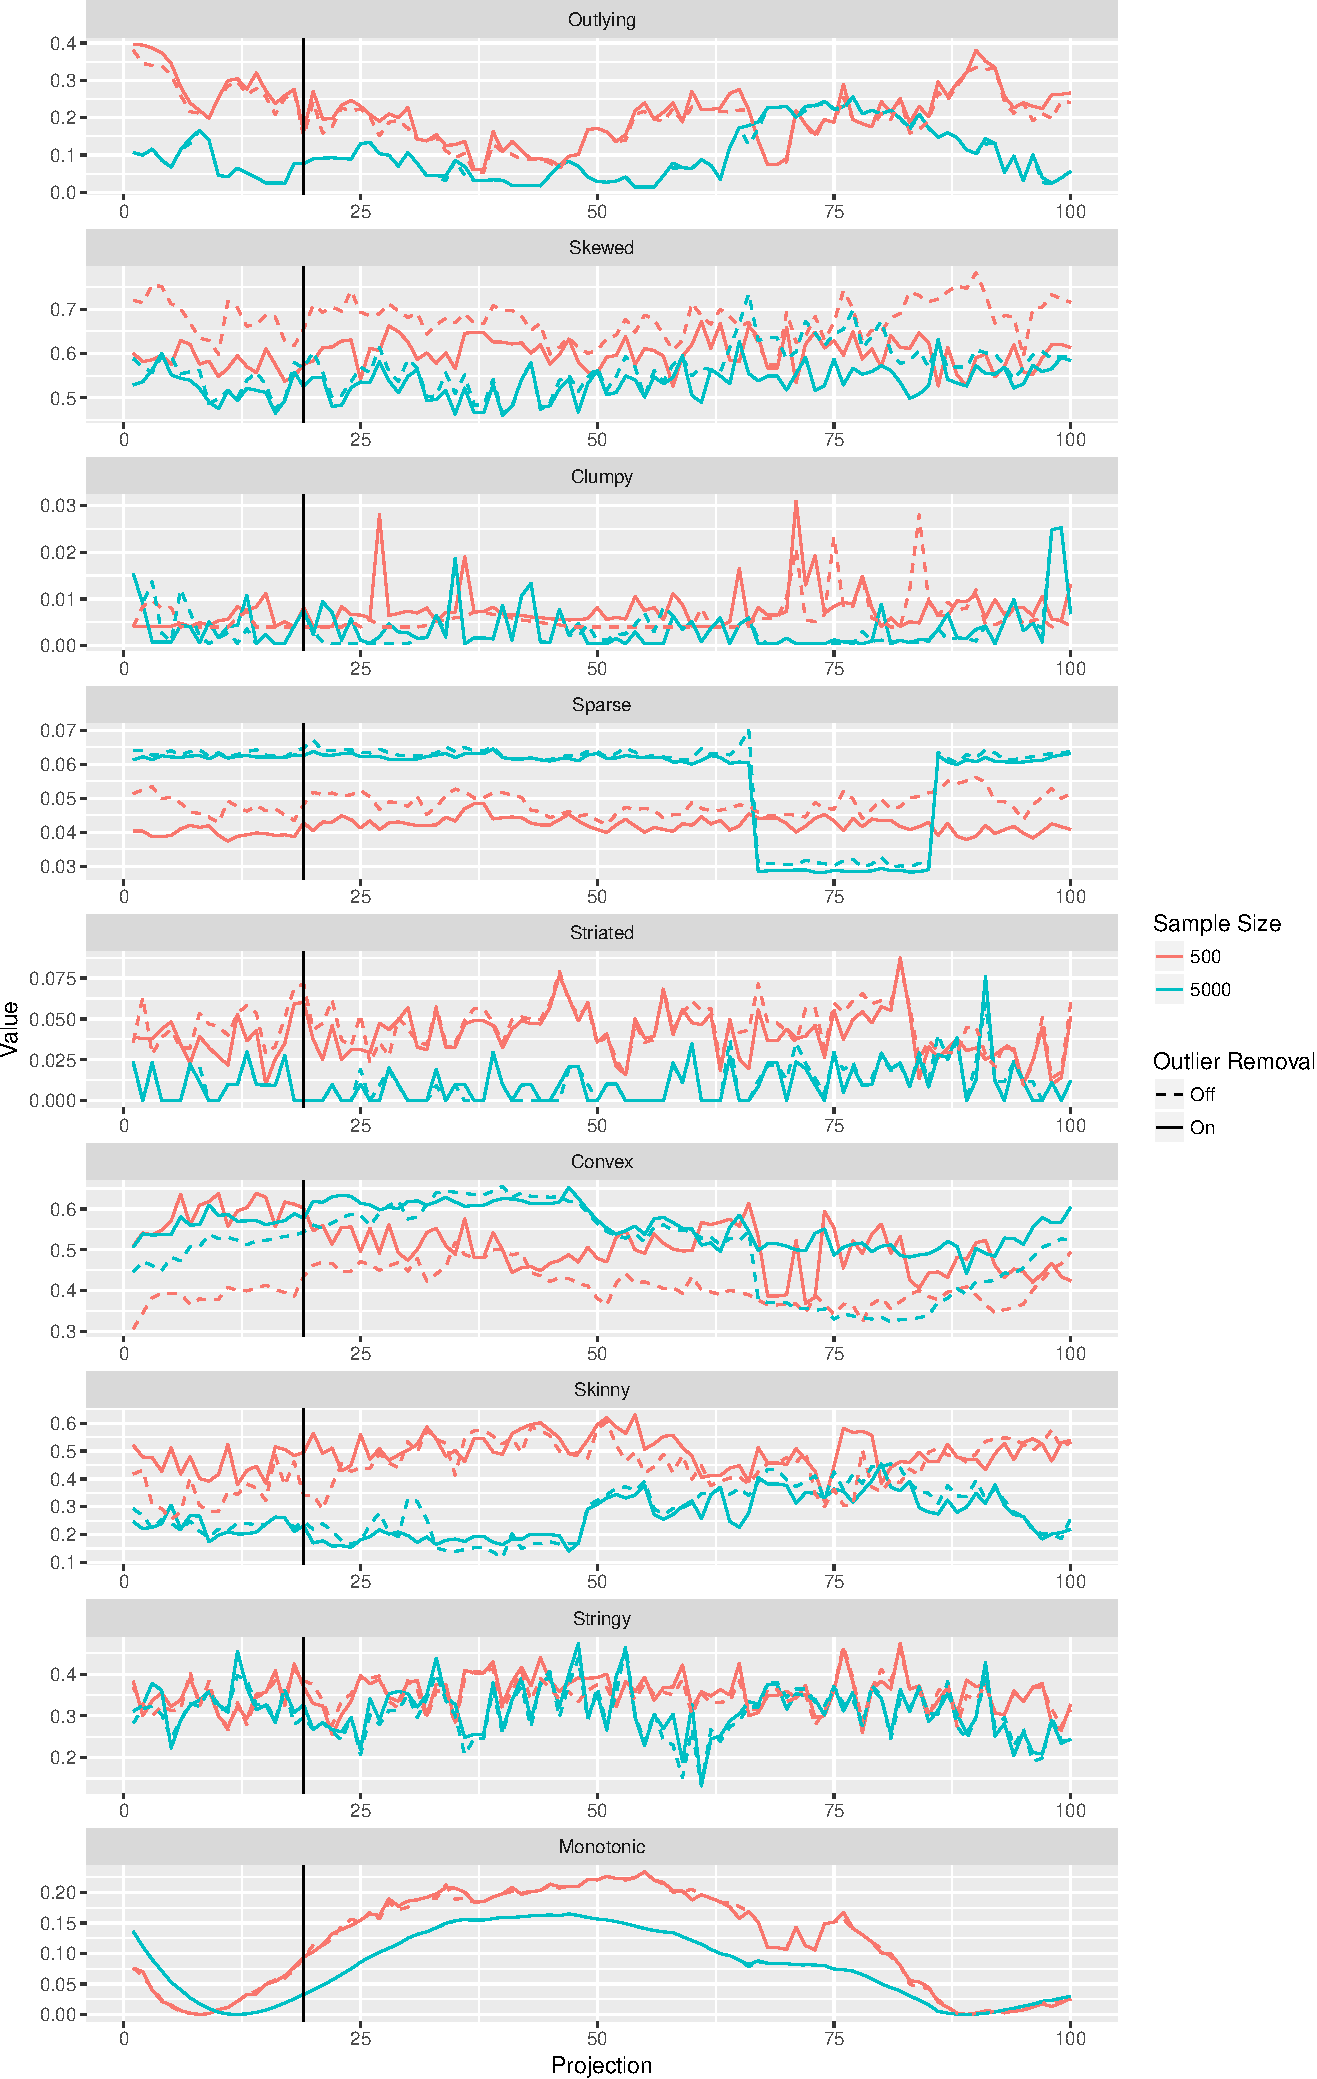
\includegraphics[width=\textwidth]{figure/scagnostics-summary-1} 

}

\caption[(ref:scagnostics-summary)]{(ref:scagnostics-summary)}\label{fig:scagnostics-summary}
\end{figure}
\end{CodeChunk}

(ref:scagnostics-summary) Summary of evolution of scagnostics measures
over 100 interpolated grand tour projections We see that three of the
considered measures, Clumpy, Sparse and Striated, are not relevant for
the considered data and projections, as the valuse are consistently low
(clearly below 0.1). The remaining measures show large variation
depending on the projection, sample size and also often strong
dependence on the outlier removal before calculation of scagnostics
measures. Moreover, we note that despite considering interpolated
projections, i.e.~a smooth transition between the randomly selected
projection planes in the grand tour, the variation of the scagnostics
measures does not follow a smooth evolution but exhibits several spikes.
This behaviour is expected to result in difficulites when using
scagnostics measures as a projection pursuit index in the context of a
dynamic guided tour. To further understand this behaviour let us study
the projected data points and also the binned version for some of the
projections exhibiting a spike. We first show in Figure ADDREF
projections t=18/19/20 of the small data set (500 data points). Not that
t=19 has been marked by a vertical line in Figure ADDREF. The left
column shows the projected data points, and the right column the binned
data used to calculate the scagnositcs measures. The scagnostics
measures in the three projections are summarised in Table ADDREF. We see
that despite similar distribution of the points in all three
projections, the outlying measure is similar for t=18 and t=20 but
jumpig down for t=19. Differences can however be observed in the binned
data (right column of Figure ADDREF), likely causing the behaviour of
the measures.

(This is blueprint of how to show scatter and binning plots but maybe
other projections will be more interesting.)

FIXME need to arrange plots better! Fix common axes for all
corresponding plots FIXME binned plot needs better formatting so we can
see relevant features easily

\begin{CodeChunk}
\begin{figure}

{\centering 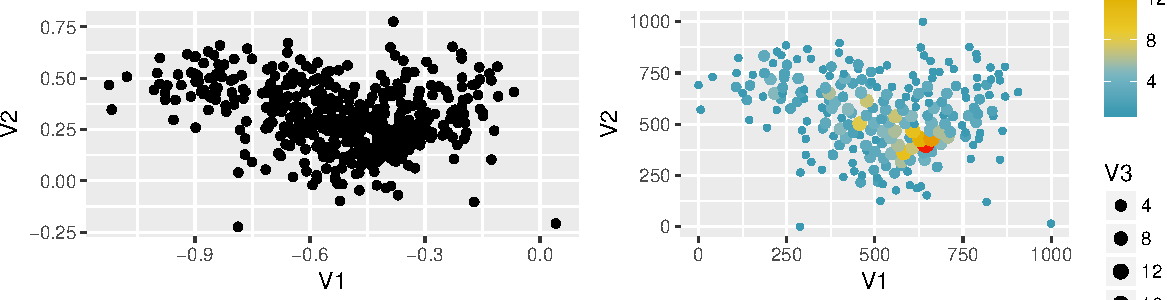
\includegraphics[width=\textwidth]{figure/scatter-binning-1} 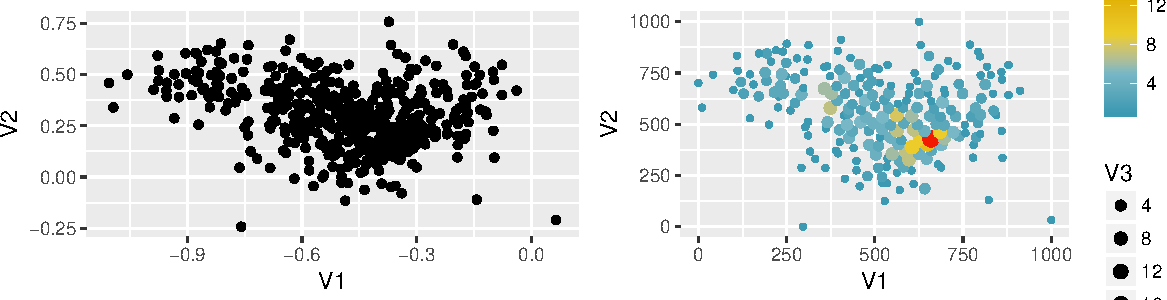
\includegraphics[width=\textwidth]{figure/scatter-binning-2} 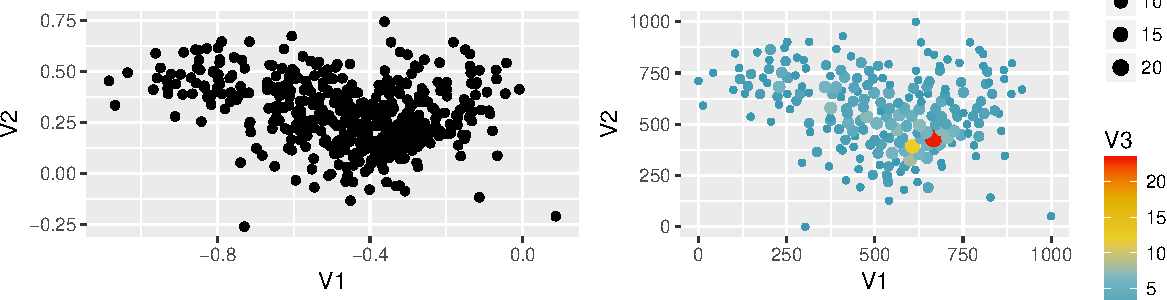
\includegraphics[width=\textwidth]{figure/scatter-binning-3} 

}

\caption[(ref:scatter-binning)]{(ref:scatter-binning)}\label{fig:scatter-binning}
\end{figure}
\end{CodeChunk}

\begin{CodeChunk}

\begin{CodeOutput}
                   s1          s2          s3
Outlying  0.275676305 0.163548110 0.270907044
Skewed    0.549038842 0.575422054 0.583569727
Clumpy    0.004123711 0.008163265 0.004175365
Sparse    0.038765964 0.042779580 0.040551326
Striated  0.059405941 0.060000000 0.037433155
Convex    0.611714549 0.602591732 0.546399191
Skinny    0.483884014 0.495557112 0.564627720
Stringy   0.424567811 0.368764181 0.329434667
Monotonic 0.077330543 0.094217913 0.103036354
\end{CodeOutput}
\end{CodeChunk}

Another consideration relevant for the purpose of the guided tour is the
computing time, as mentioned above it may limit the tour display to
previously recorded tours. We study here the computing time depending on
the sample size with and without the outlier removal when calculating
the measures. Figure ADDREF shows this variation for 3 different sample
selections. The time is measured over the 100 projections shown before
and is the sum of computing time for projecting the data and calculating
the scagnostics measures on the projected data. We see that overall the
outlier removal increases the runtime by about a factor two. However we
have seen above that skipping the step of outlier removal often leads to
very different values of some of the scagnostics measures. (What to do
with this information? Should not skip this step?) Interestingly the
computing times are longest for intermediate sample sizes of a few
hundred data points, and converge to lower run times for larger samples.
This is because the binning of the input data is much faster than the
computation of the measures which is increased for smaller samples.

\begin{CodeChunk}
\begin{figure}

{\centering 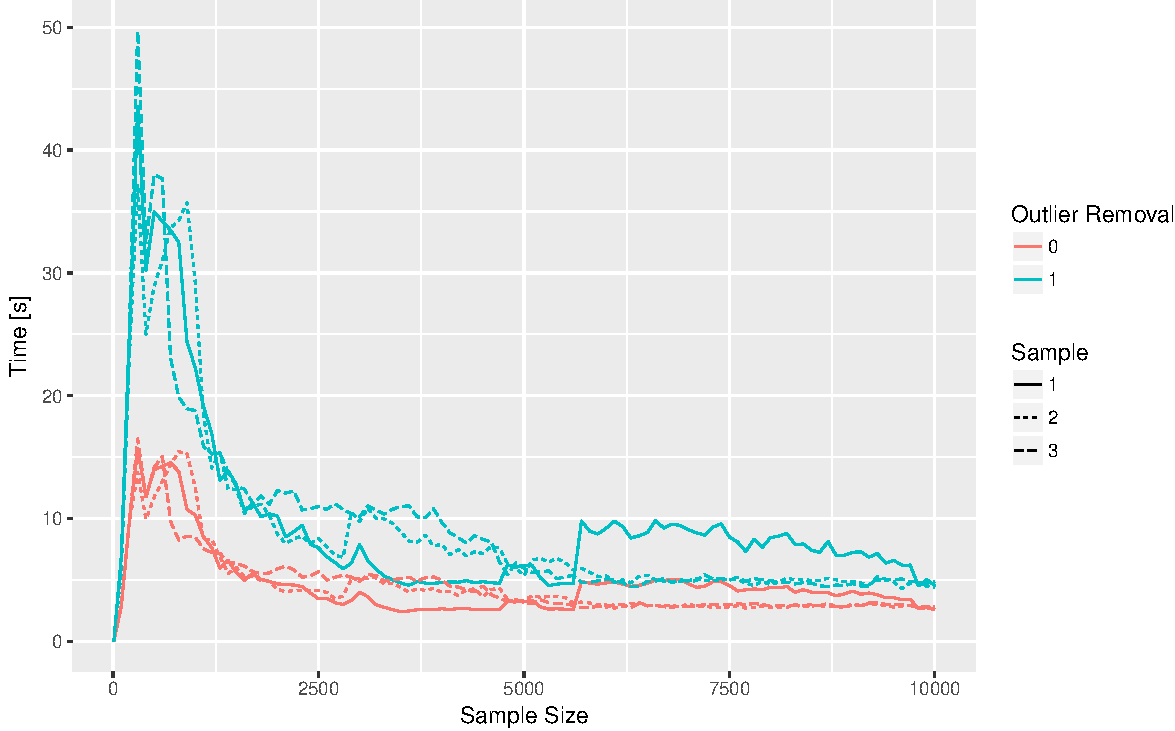
\includegraphics[width=\textwidth]{figure/scagnositcs-timing-1} 

}

\caption[(ref:scagnostics-timing)]{(ref:scagnostics-timing)}\label{fig:scagnositcs-timing}
\end{figure}
\end{CodeChunk}

\subsection{Smooth transitions}\label{smooth-transitions}

We next turn to the question of how we can obtain smooth transitions of
the scagnostics measures. (Below just an example of using ggplot
smoothing to display what kind of behaviour we want to find. It follows
the general trend without capturing the spikes.)

\begin{CodeChunk}
\begin{figure}

{\centering 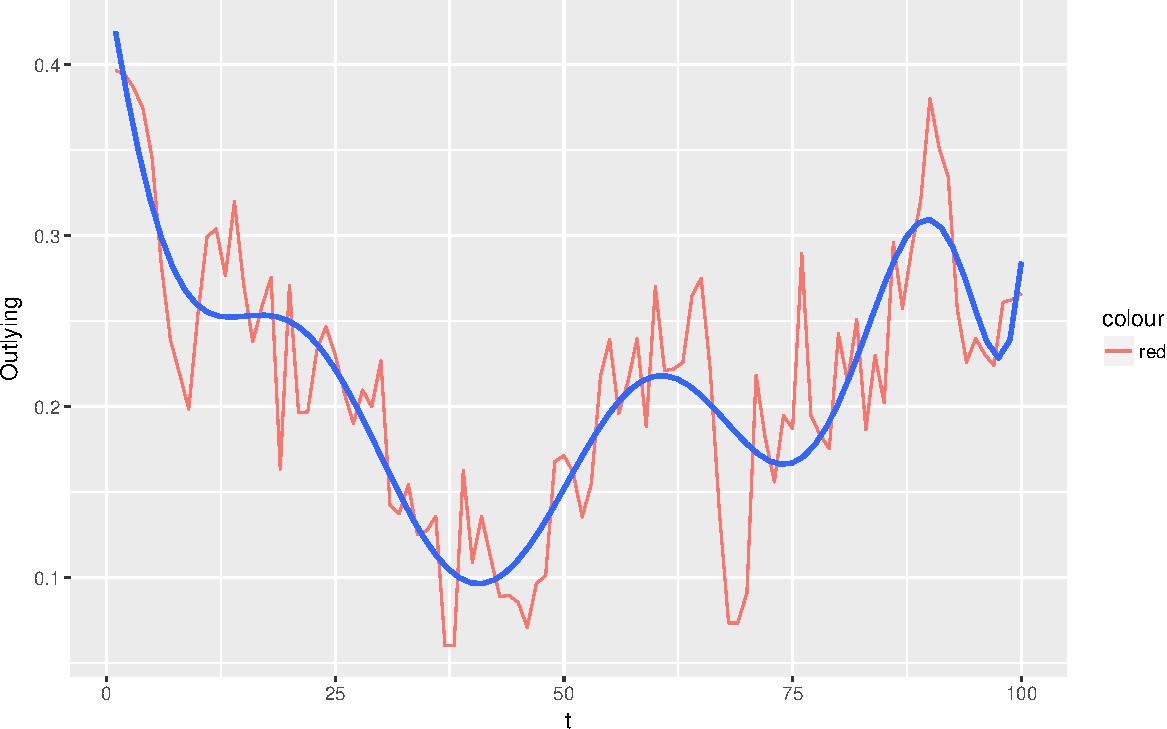
\includegraphics[width=\textwidth]{figure/smoothing-1} 

}

\caption[(ref:smooting)]{(ref:smooting)}\label{fig:smoothing}
\end{figure}
\end{CodeChunk}

Want to explore jittering either the projection or the points, but this
does not give the desired smooth behaviour (why?) Maybe show how it
compares to the sketch of smooth polynomial function? Select parameters
from previous study without including the detailed plots here..

\subsubsection{Binning in high
dimensions?}\label{binning-in-high-dimensions}

\subsubsection{Outlier removal before
binning?}\label{outlier-removal-before-binning}

\subsection{Test with guided tour}\label{test-with-guided-tour}

try out scagnostics measures as guided tour index

Example below uses Convex as index function. We show the evolution of
the index on the interpolated guided tour (top) and on the selected
planes without interpolation (bottom). Note that the interpolated
projections do not smoothly increase the index value from one selected
plane to the next, but shows the unstable nature of the index
computation.

\begin{CodeChunk}
\begin{figure}

{\centering 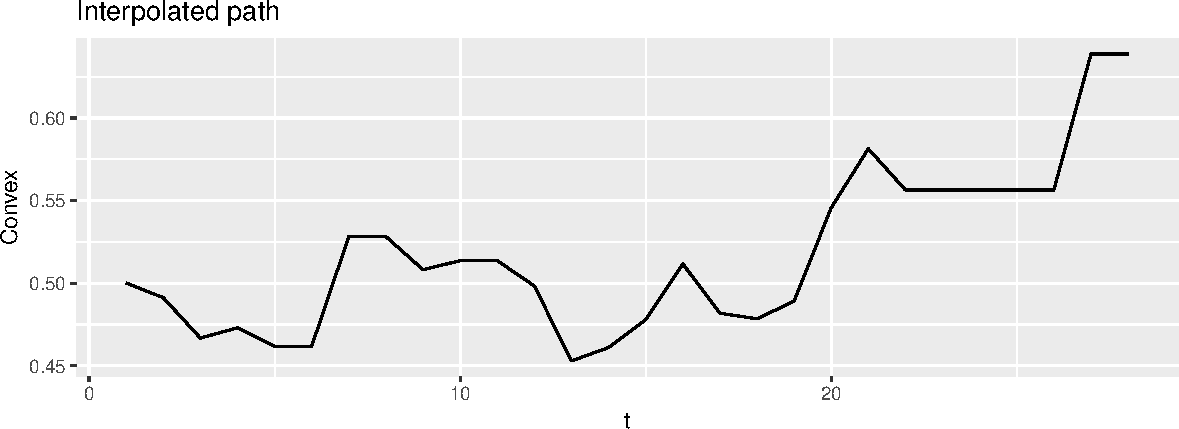
\includegraphics[width=\textwidth]{figure/guided-tour-plot-1} 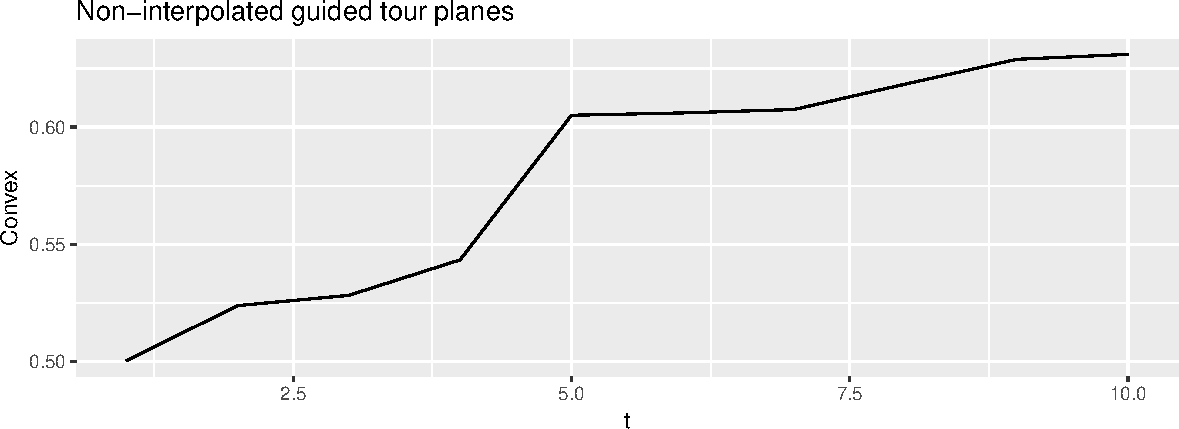
\includegraphics[width=\textwidth]{figure/guided-tour-plot-2} 

}

\caption[(ref:guided-tour-plot)]{(ref:guided-tour-plot)}\label{fig:guided-tour-plot}
\end{figure}
\end{CodeChunk}

Figure (ref:guided-tour-scatter) compares the scatter plots (left
unbinned, right binned) of the start projection, the projection with the
lowest index value (t=19 of the interpolated projections) and the final
projection (t=28).

\begin{CodeChunk}
\begin{figure}

{\centering 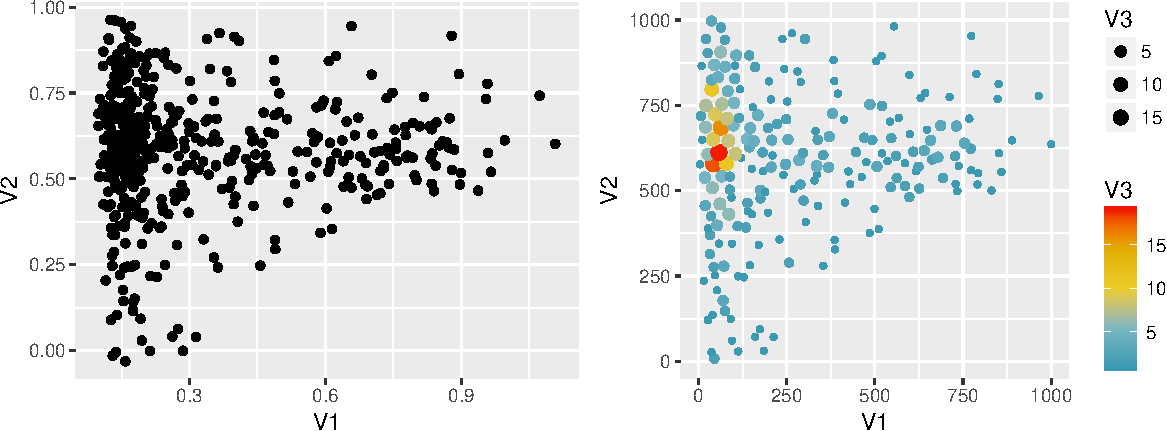
\includegraphics[width=\textwidth]{figure/guided-tour-scatter-1} 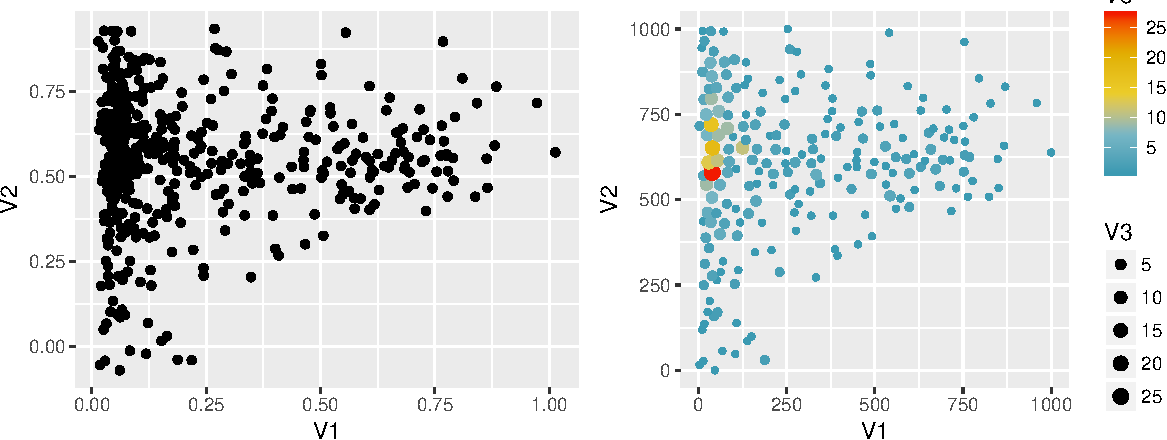
\includegraphics[width=\textwidth]{figure/guided-tour-scatter-2} 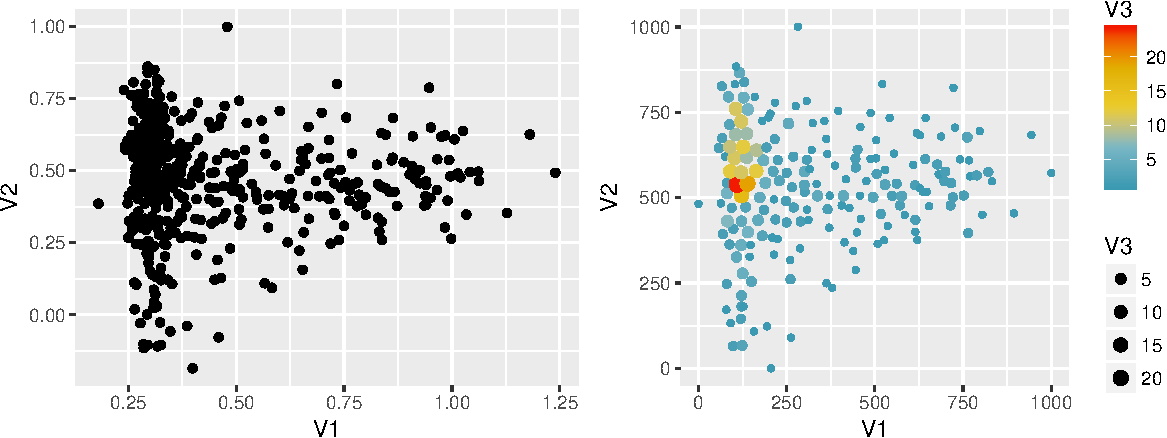
\includegraphics[width=\textwidth]{figure/guided-tour-scatter-3} 

}

\caption[(ref:guided-tour-scatter)]{(ref:guided-tour-scatter)}\label{fig:guided-tour-scatter}
\end{figure}
\end{CodeChunk}

show computing time? for each index as function of sample size? (long to
prepare such a plot..)

\subsection{Additional indices to
consider}\label{additional-indices-to-consider}

FIXME load Katrins package and try the index functions she implemented

Additions to the standard scagnostics measures have been implemented in
the package mbgraphics, based on splines (spline2d) and distance
correlation (dcor2d). Give definitions here.. We repeat the study from
before, we first test in Figure ADDREF the behaviour of the index values
over 100 interpolated projections that are randomly selected via the
grand tour algorithm. Note that here the measures are calculated on
non-binned data. The observed behaviour is smooth (much in contrast to
the behaviour of the scagnostics measures) and we next test the
behaviour in a guided tour, comparing again also the first and final
projection. (which index to select, will try both below\ldots{}) It
seems they both maximise correlation, this might not be too useful
here\ldots{}

\begin{CodeChunk}
\begin{figure}

{\centering 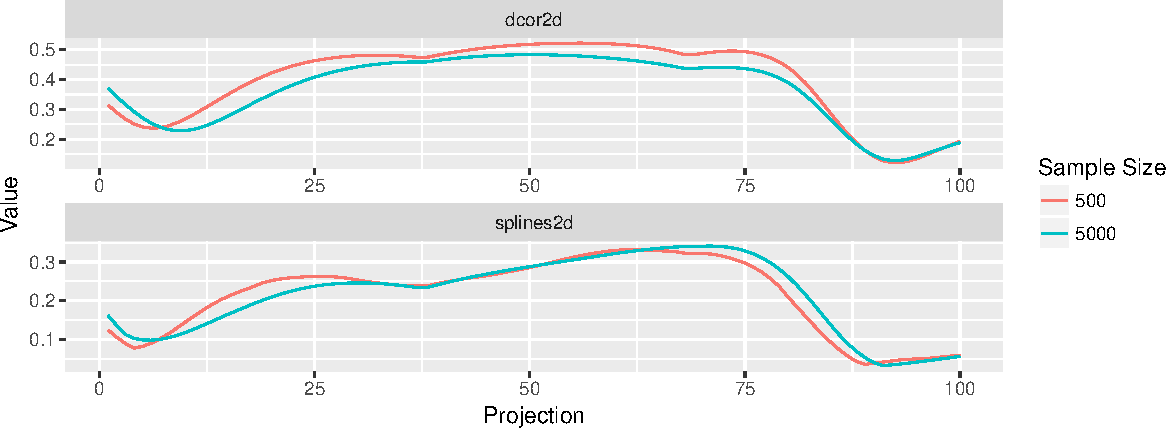
\includegraphics[width=\textwidth]{figure/mbgraphics-indices-1} 

}

\caption[(ref:mbgraphics-indices)]{(ref:mbgraphics-indices)}\label{fig:mbgraphics-indices}
\end{figure}
\end{CodeChunk}

\begin{CodeChunk}
\begin{figure}

{\centering 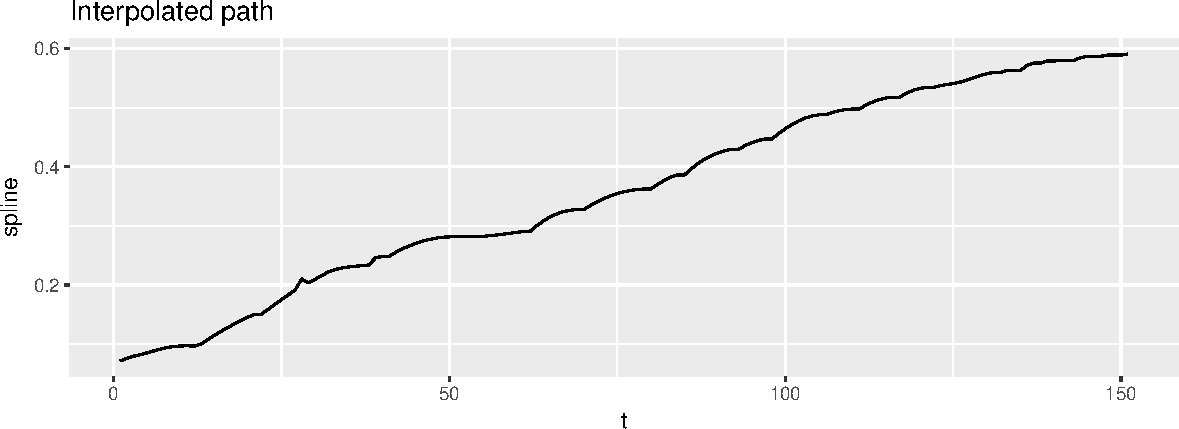
\includegraphics[width=\textwidth]{figure/guided-spline2d-plot-1} 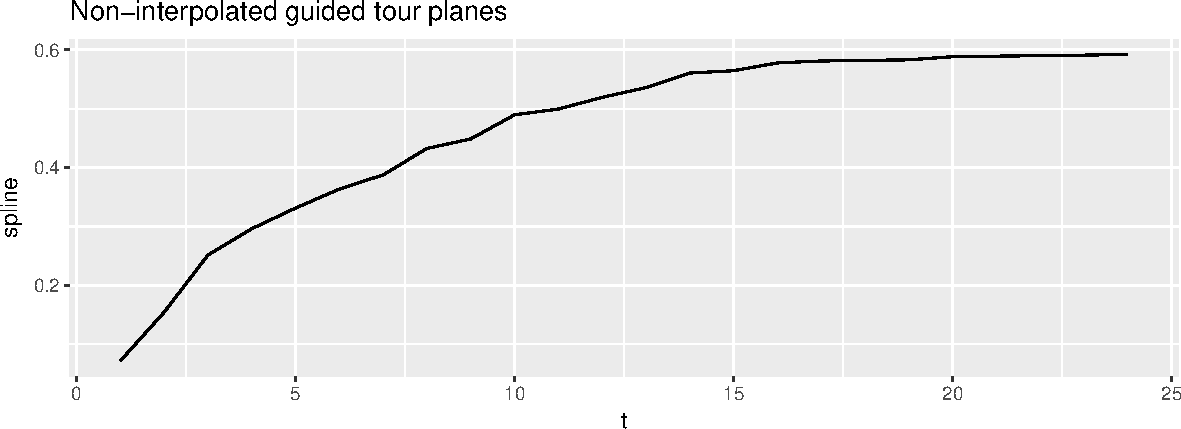
\includegraphics[width=\textwidth]{figure/guided-spline2d-plot-2} 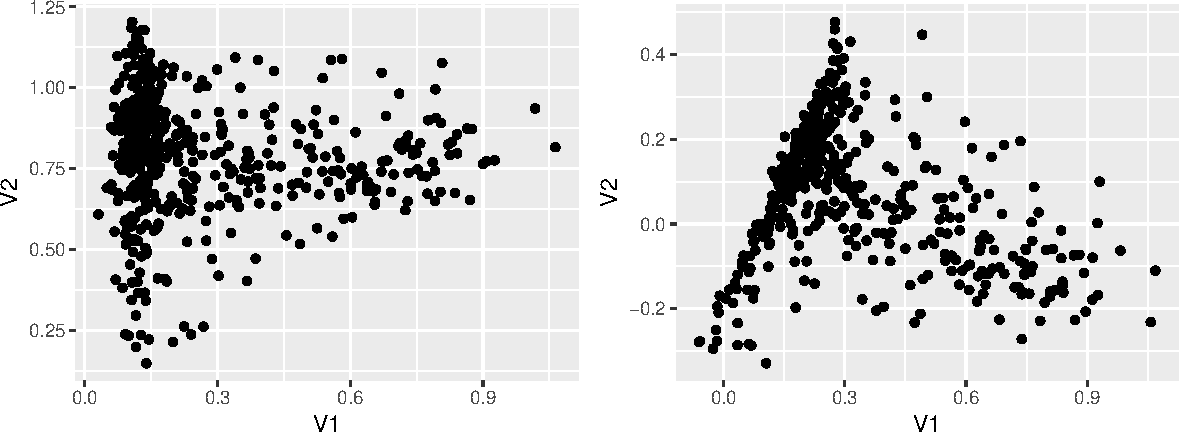
\includegraphics[width=\textwidth]{figure/guided-spline2d-plot-3} 

}

\caption[(ref:guided-spline2d-plot)]{(ref:guided-spline2d-plot)}\label{fig:guided-spline2d-plot}
\end{figure}
\end{CodeChunk}

\begin{CodeChunk}

\begin{CodeOutput}
            [,1]        [,2]
[1,]  0.47851413 -0.54459454
[2,]  0.01632788 -0.00642453
[3,]  0.20956852 -0.15615632
[4,] -0.21613392  0.22043552
[5,] -0.26952654  0.31203441
[6,] -0.27310129  0.26333539
[7,] -0.72999721 -0.68094632
\end{CodeOutput}
\begin{figure}

{\centering 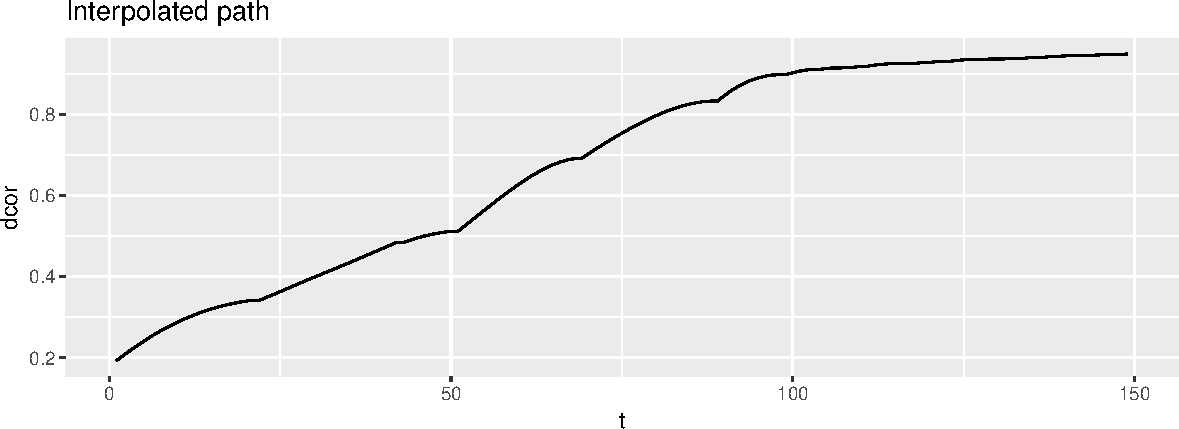
\includegraphics[width=\textwidth]{figure/guided-dcor2d-plot-1} 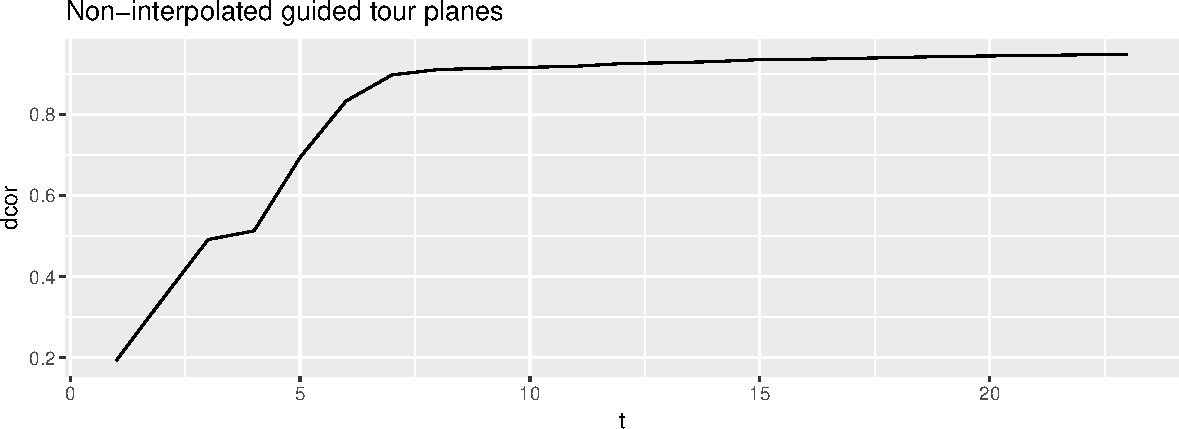
\includegraphics[width=\textwidth]{figure/guided-dcor2d-plot-2} 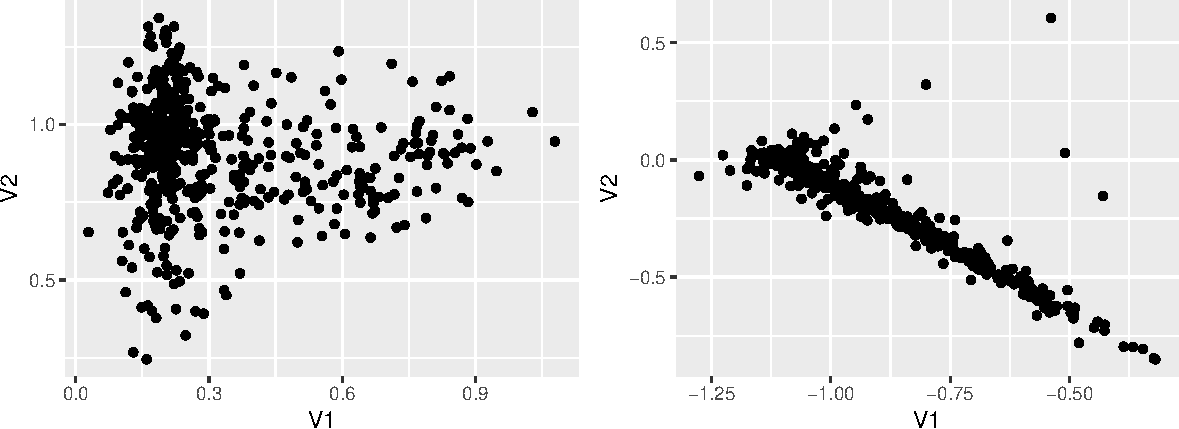
\includegraphics[width=\textwidth]{figure/guided-dcor2d-plot-3} 

}

\caption[(ref:guided-dcor2d-plot)]{(ref:guided-dcor2d-plot)}\label{fig:guided-dcor2d-plot}
\end{figure}
\end{CodeChunk}

maybe move timing to the end, add also these indices in the same plot
(instead of testing several samples, behaviour anyway similar)



\end{document}

